\chapter{\textit{Data Preparation}}
\label{chap:data_prep}


% MISSING VALUES
\section{\textit{Missing values} (Ambos)}
\label{chap3:missing_values}

Como foi referido no capítulo \ref{chap2:dataset} o \textit{dataset} não tem valores em falta, por isso tivemos que os criar artificialmente. Para simular valores em falta foi criado um programa que a partir do \textit{dataset} original substituía elementos aleatórios de categorias aleatórias por um valor vazio "None", e a partir daí foram feitos métodos para tentar lidar com estes valores em falta.

\subsection{Método 1 - Substituir pelo valor mais frequente (Vicente)}
\label{chap3:metodo1}

Uma forma comum de lidar com elementos em falta é substituir o valor em falta pelo valor mais frequente na sua categoria especifica, e foi isso que foi implementado neste trabalho. Esta forma foi implementada tal como diz no seu nome, primeiro é calculado e guardado o valor mais frequente de cada categoria, após isso percorremos o \textit{dataset} todo, e se for encontrado um valor em falta, elemento com valor "None", esse elemento é substituído pelo valor mais frequente da categoria a que pertence e a função continua até acabar de percorrer o \textit{dataset}.

\subsection{Método 2 - Fill Missing Values with Mean and Mode (João)}
\label{chap3:metodo2}

Este método lida valores em falta preenchendo-os com a média (em caso de dados numéricos) ou a moda (em caso de dados categóricos) da coluna correspondente.

Este método não remove dados e garante um valor adequado para cada dado em falta de acordo com o seu tipo, sendo um bom compromisso.



% ====================
% DATA NORMALIZATION
% ====================

\section{\textit{Data Normalization}, \textit{Discretization} e \textit{Reduction} (Ambos)}
\label{chap3:data}

\subsection{\textit{Data Normalization} (João)}
\label{chap3:data_norm}

A normalização dos dados é fundamental na preparação algoritmos de aprendizagem automática, especialmente aqueles sensíveis à escala das variáveis como \textit{K-Nearest Neighbors} ou \textit{Multi-Layer Perceptron}.

Foram implementados dois métodos de normalização:

\begin{itemize}
    \item \textbf{\textit{Min-Max Normalization}:} Transforma os valores, trazendo-os para o intervalo \([0, 1]\), segue a seguinte fórmula:
    \[
    x' = \frac{x - x_{min}}{x_{max} - x_{min}}
    \]
    
    onde:
    \begin{itemize}
        \item \( x \) é o valor original.
        \item \( x_{min} \) e \( x_{max} \) são, respetivamente, o menor e o maior valor na coluna.
        \item \( x' \) é o valor normalizado.
    \end{itemize}

    \item \textbf{\textit{Z-Score Normalization}:} Transforma os dados para que tenham uma média de 0 e um desvio padrão de 1. Segue a fórmula:
    \[
    z = \frac{x - \mu}{\sigma}
    \]
    onde:
    \begin{itemize}
        \item \( x \) é o valor original.
        \item \( \mu \) é a média da coluna.
        \item \( \sigma \) é o desvio padrão da coluna.
        \item \( z \) é o valor normalizado.
    \end{itemize}
\end{itemize}

Ambos os métodos foram implementados e podem ser selecionados conforme a necessidade do modelo ou a natureza dos dados.


\subsection{\textit{Data Discretization} (Vicente)}
\label{chap3:data_disc}

Como referido no capítulo \ref{chap2:dataset}, o \textit{dataset} contem inconsistências, e com o uso do \textit{data discretization} é possível removê-las completamente. Para a discriminação dos dados fui ver quais categorias é que tinham o maior número de respostas diferentes, após essa revisão conclui que as categorias 'Height (cm)', 'Weight (kg)', 'BMI','Alcohol Consumption', 'Fruit Consumption', 'Green Vegetables Consumption' e 'FriedPotato Consumption' eram as que mais sofriam de um número exagerado de respostas diferentes.

Para resolver esse problema defini limites para cada uma das categorias e atualizei os seus valores, como, por exemplo, no excerto de código \ref{codigo:data_disc}. A única categoria faço algo mais é o 'BMI', pois como tinha dito no capítulo \ref{chap2:dataset} este tem um pequeno desvio do seu valor real, logo, antes de o categorizar calculo o valor real do BMI através do peso e altura da pessoa.

\begin{lstlisting}[caption={Excerto de código utilizado para substituir todos os valores numericos da categoria 'Height (cm)' por valores categoricos.}, language=Python, label={codigo:data_disc}]
# ALTURA -> em vez de usar os valores verdadeiros da altura, reduzir para algumas categorias genericas
for i in range(len(dataset[11])):
    if dataset[11][i] < 150: # +1.5m
			dataset[11][i] = "<150"
    elif dataset[11][i] >= 150 and dataset[11][i] <=160: # entre 1.5 e 1.6 m
			dataset[11][i] = "150-160"
    elif dataset[11][i] > 160 and dataset[11][i] <=170: # entre 1.6 e 1.7 m
			dataset[11][i] = "161-170"
    elif dataset[11][i] > 170 and dataset[11][i] <=180: # entre 1.7 e 1.8 m
			dataset[11][i] = "171-180"
    elif dataset[11][i] > 180 and dataset[11][i] <=190: # entre 1.8 e 1.9 m
			dataset[11][i] = "181-190"
    elif dataset[11][i] > 190 and dataset[11][i] <=200: # entre 1.9 e 2.0 m
			dataset[11][i] = "191-200"
    else: # +2.0m
			dataset[11][i] = ">200"
\end{lstlisting}

\begin{figure}[H]
    \centering
    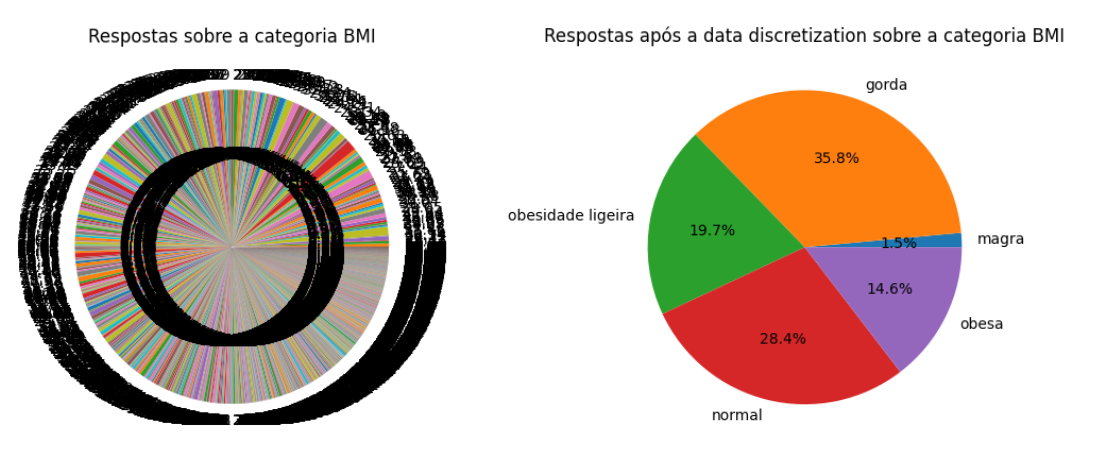
\includegraphics[scale=0.45]{BMI.png}
    \caption{Valores da categoria 'BMI' antes e depois da aplicação da discretização dos dados.}
    \label{fig:bmi}
\end{figure}


\subsection{\textit{Data Reduction} (Vicente)}
\label{chap3:data_redu}

A redução dos dados foi feita através 3 formas diferentes de redução: eliminação de duplicados, eliminação de categorias inúteis para o objetivo e junção de categorias.

A eliminação de duplicados é bastante óbvia, cada vez que a função de redução é chamada é verificado se o \textit{dataset} tem elementos duplicados, se tiver serão removidos.

De seguida foi feita a remoção das categorias 'General Health' e 'Checkup', pois como o objetivo é tentar prever se um indivíduo tem ou não problemas cardíacos, categorias como as mencionadas não irão influenciar no objetivo. A categoria 'General Health' é uma categoria de opinião sobre a saúde geral do próprio individuo, não tem nenhuma relação com doenças cardíacas. A categoria 'Checkup', apesar da sua temática médica, é apenas uma verificação de quando é que foi a última vez que o individuo foi ao médico, o que não influencia em doenças cardíacas.

O passo principal nesta fase foi a redução das categorias de consumo para uma categoria nova 'qualidade da dieta' (categorias 16, 17, 18 e 19 como referido no capítulo \ref{chap2:dataset}). Para obter criar essa nova categoria decidi calcular o "valor" da dieta de cada indivíduo, para tal somei os valores das categorias 17 e 18 e subtrai as categorias 16 * 4 (a categoria 16 é multiplicada por 4 para dar mais valor no cálculo, pois os seus valores estão só entre 0 e 30) e 19, como indicado no excerto de código \ref{codigo:dieta}. Após isso calculei a média dos valores obtidos e o desvio padrão e defini os parâmetros da nova categoria com eles, após isso verifiquei cada valor de forma semelhante a \ref{codigo:data_disc} e criei a nova categoria como é mostrado na figura \ref{fig:dieta}.

\begin{lstlisting}[caption={Excerto de código utilizado para calcular o valor da dieta a partir das categorias de consumo}, language=Python, label={codigo:dieta}]
# calculo para obter o valor da dieta da pessoa:
# valor_da_dieta = fruta + vegetais - alcool*4 - batata
numeros = dataset.iloc[:, 14] + dataset.iloc[:, 15] - dataset.iloc[:, 13]*4 - dataset.iloc[:, 16]
    
# calcular a media e o desvio
media = np.mean(numeros)
desvio = np.std(numeros)*0.5
    
# calcular os valores para as condicoes de cada label, usando a media e um desvio
valores_correspondentes = [media - 3 * desvio, media - 2 * desvio, media - desvio, media, media + desvio, media + 2 * desvio, media + 3 * desvio]
\end{lstlisting}

\begin{figure}[H]
    \centering
    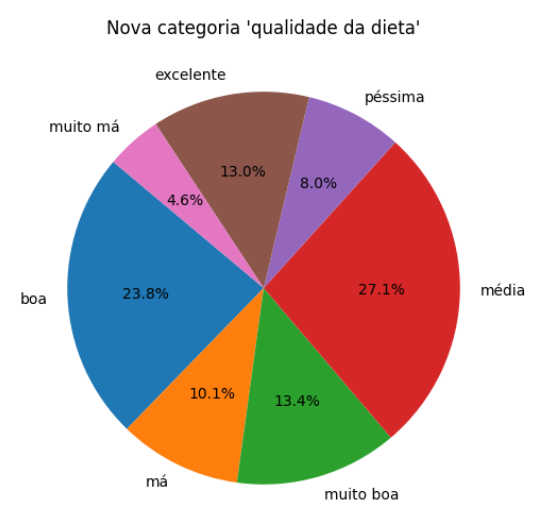
\includegraphics[scale=0.5]{dieta.png}
    \caption{Nova categoria 'qualidade da dieta' feita através das categorias de consumo.}
    \label{fig:dieta}
\end{figure}

Além destas também pensei em eliminar as categorias 'Height (cm)' e 'Weight (kg)' e deixar apenas o 'BMI', no entanto, achei melhor deixar estar ambas as categorias, pois com o BMI não podemos saber concretamente a altura e peso e apenas com o ele os modelos poderiam obter piores resultados, pois podem existir correlações relevantes entre altura e peso que eu não tenha conhecimento.